\scalebox{1}{
	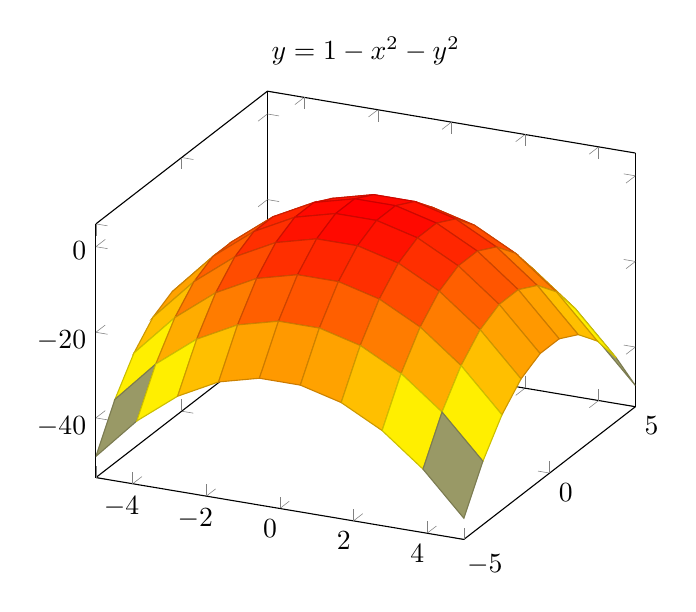
\begin{tikzpicture}
		\begin{axis}[
				title={$y=1-x^2-y^2$},
			]
			\addplot3[surf,samples=10]{1-x^2-y^2};
		\end{axis}
	\end{tikzpicture}
	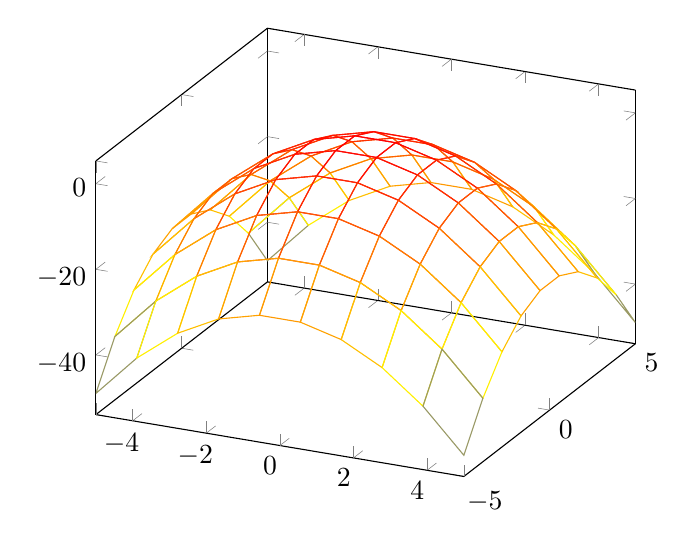
\begin{tikzpicture}
		\begin{axis}
			\addplot3[mesh,samples=10]{1-x^2-y^2};
		\end{axis}
	\end{tikzpicture}
}
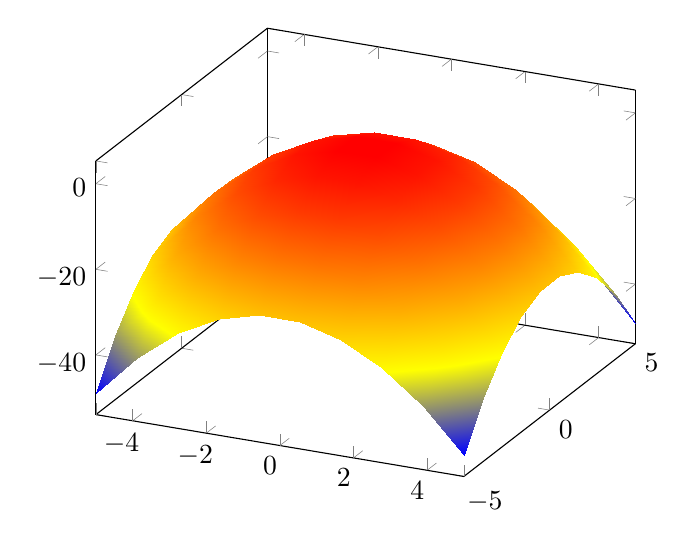
\begin{tikzpicture}
	\begin{axis}
		\addplot3[surf,samples=10,shader=interp]{1-x^2-y^2};
	\end{axis}
\end{tikzpicture}
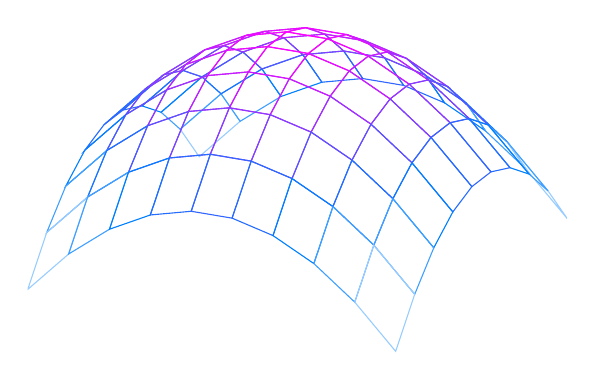
\begin{tikzpicture}
	\begin{axis}[colormap/cool, hide axis]
		\addplot3[mesh,samples=10]{1-x^2-y^2};
	\end{axis}
\end{tikzpicture}

\subsubsection{Меняем угол просмотра, вращаем график}

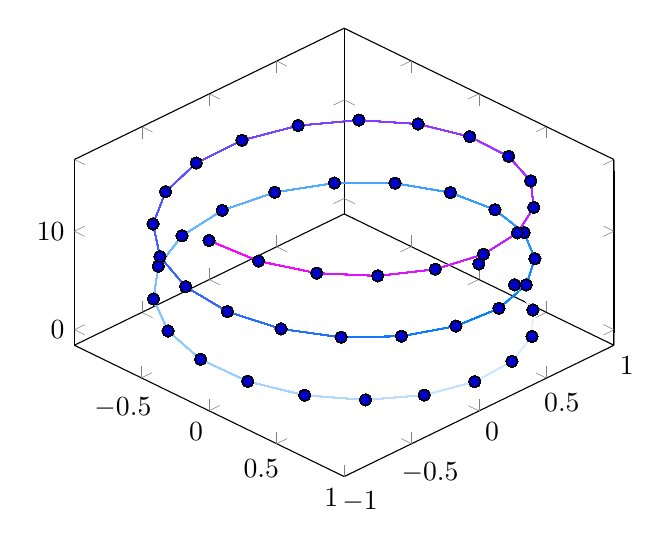
\begin{tikzpicture}
	\begin{axis}[colormap/cool, view={45}{45}]
		\addplot3+[domain=0:5*pi,mesh,samples=50]
		({sin(deg(x))},
		{cos(deg(x))},
		{x});
	\end{axis}
\end{tikzpicture}
